\documentclass{article}
\usepackage[utf8]{inputenc}
\usepackage{cite}
\usepackage{graphicx}
\usepackage{float}
\usepackage{amssymb}
\usepackage{amsmath}
\usepackage{cancel}
\usepackage{float}
\usepackage{listings}
\usepackage{hyperref}
\usepackage[]{algorithm2e}
\usepackage{xcolor}

 
\definecolor{codegreen}{rgb}{0,0.6,0}
\definecolor{codegray}{rgb}{0.5,0.5,0.5}
\definecolor{codepurple}{rgb}{0.58,0,0.82}
\definecolor{backcolour}{rgb}{0.95,0.95,0.92}
\definecolor{codeblue}{rgb}{0.1,0.1,0.95}
 
\lstdefinestyle{mystyle}{
    backgroundcolor=\color{backcolour},   
    commentstyle=\color{codegreen},
    keywordstyle=\color{magenta},
    numberstyle=\tiny\color{codegray},
    stringstyle=\color{codepurple},
    basicstyle=\ttfamily\footnotesize,
    breakatwhitespace=false,         
    breaklines=true,                 
    captionpos=b,                    
    keepspaces=true,                 
    numbers=left,                    
    numbersep=5pt,                  
    showspaces=false,                
    showstringspaces=false,
    showtabs=false,                  
    tabsize=2
}
 
\lstset{style=mystyle}

\newtheorem{theorem}{Theorem}

\newcommand*{\QEDA}{\hfill\ensuremath{\blacksquare}}%
\newcommand*{\QEDB}{\hfill\ensuremath{\square}}%

\title{[Insert Name of the Software]}
\author{GISC}
\date{\today}

\begin{document}

\maketitle

\section{Abstract}

Under Consctruction


\section{Introduction}

In this text it will be summarized the pseudocodes and the general scheme of the [insert name here] package created by the Interdisciplinary Group of Complex Systems....

\section{General Scheme of the Package}

The [name] is written in Python Language because of it simple syntax and the vast amount of packages developed by the community. In this package we take advantage of the Object Oriented Programming (OOP) feature of Phyton. The main idea is to generate a robust and easier to work package, that could be improved by the community of complex systems. In the following image is summarized the scheme of the package 

\begin{figure}
    \centering
    \includegraphics[width=0.9\textwidth]{DiagramPackage.pdf}
    \caption{General Scheme of the package [name]. The red arrows means that \textit{it is inherit from}. The black arrows means that \textit{it is imported from}. The black boxes correspond to the \textit{wrappers}. The blue boxes correspond to \textit{class or objects}. The rec circles correspond to the \textit{main classes}, it means the parent classes.}
    \label{scheme}
\end{figure}

In the package the principal classes that are used are the class \textit{Node} and the class \textit{Network}. All the other classes inherit from these basic objects. The blue boxes correspond to the daughter classes of Node and Network. The black boxes correspond to the wrappers, it means that import all the objects that correspond to certain functionality. In our case we classified the classes in: topologies, to those codes that give the topology to the graph/network and dynamics, to those codes that correspond to the dynamics, independently of the topology of the graph/network used. The Wrapper black box, what it does is import Topology.py and Dynamics.py and have a main code. The dotted boxes correspond to the non-implemented classes or codes but are planned to be implemented in the future. 

\section{Parents Classes}

In this section it will be shown the already implemented classes \textit{Node} and \textit{Network}. 

\subsection{Node Class}

The node class have only two methods. The constructor \textit{init}, which recieve a pointer of argument $*argv$. In this case it only need the first argument $argv[0]$, which is a list of integers that correspond to the connections \textit{.cnx} of the node. The other methods corresponds to the \textit{str}, which is in charge of the printing format. 

\begin{lstlisting}[language=Python, caption=Node Class]
import numpy as np 

class node:

    def __init__(self, *argv):
        """Constructor"""
        self.cnx = argv[1] # Lista de vecinos
        

    def __str__(self):
        return "Conexiones: {}".format(self.cnx)
\end{lstlisting}

For example: 

\begin{lstlisting}[language=Python, caption=Example Node Class]
    nodo = node([1,2,3,4])
    nodo2 = node([5,6])
    print("Nodo1 :"+str(nodo))
    print("Nodo2 :"+str(nodo2))
--------------------------------------------------------------------
    Nodo1 :Conexiones: [1, 2, 3, 4]
    Nodo2 :Conexiones: [5, 6]
\end{lstlisting}

\subsection{Network Class}

The network class is a little bit more complex because it contains some of the methods to draw and export the topologies of the networks. First, we import the libraries \textit{matplotlib}  and \textit{networkx} to help us to plot the networks. The library \textit{numpy} is imported to help us with some mathematical operation that we could need. We also import the class \textit{Node} because a network contain a list of nodes.

Now, let us focus on the implemented methods. First, the constructor have only one input \textit{NumeroNodos}, which corresponds to the total number of nodes that our network is going to include. The constructor define two characteristics of the class: \textit{self.N}, the number of nodes and \textit{self.nodes}, the list of objects \textit{nodes}. For the characteristics \textit{self.nodes} it is called the method \textit{self.completeGraph()}, which return a list of nodes that all are connected between them (Complete Graph). The next method corresponds to the \textit{adjacentMatrix}, which create the adjacent matrix associated to the network. Next, the \textit{plotAdjacentMatrix} is a method that obtain the adjacent matrix and it create a plot of the graph as is shown in the Figure. \ref{circularGraph}. Finally, the method \textit{adjacentMatrixFile}, which create an adjacent matrix and export it in a data file to be used by another software to plot it like Mathematica.

\begin{lstlisting}[language=Python, caption= Network Class]
from Node import node
import numpy as np
import matplotlib.pyplot as plt
import networkx as nx

class network():

    def __init__(self, NumeroNodos):
        """Constructor"""
        self.N = NumeroNodos
        self.nodes = self.completeGraph()
        

    def completeGraph(self):
        # Method that create a complete graph. 
        # It return a list of objects node.

        nodesList = [] # Create an empty list
        nodeT= self.N # Define the total number of nodes
        for i in range(nodeT):
            nodesList.append( node([x for x in range(nodeT)  if x != i])) 
        # Append an object node, that is connected with 
        # all the other nodes except itself, at each 
        # iteration
        return nodesList
    
    def adjacentMatrix(self):
        # Method to create the adjacent matrix of the
        # network. It return a list of list (matrix).

        totalN = self.N # Total number of nodes
        matrix = np.zeros((totalN, totalN)) 
        # Initialize a matrix N x N of zeros
        for i in range(totalN):
            nodeaux = self.nodes[i]
            for j in nodeaux.cnx:
                matrix[i][j] = 1      
        # For each node i, at j an integer in the list 
        # of connections of the node it is put a 1 in 
        # the position matrix[i,j] s
        return matrix

    def plotAdjacentMatrix(self):
        # Method that plot the network. It return an
        # image of the topology of the network.

        matrix = self.adjacentMatrix() 
        # Create the adjacent matrix of the network
        rows, cols = np.where(matrix == 1) 
        # Get all the rows and columns with a number 1
        edges = zip(rows.tolist(), cols.tolist()) 
        # Create a list of edges of the form (row, col)
        gr = nx.Graph() 
        # Initialize the graph
        gr.add_edges_from(edges)
        # Add the edges to graph
        nx.draw_circular(gr, node_size=10)
        # Define the characteristics of the plot
        plt.show() 

    def adjacentMatrixFile(self, fileName):
        # Method to export a file with the adjacent 
        # matrix. 
        # Input: Name of the file.
        # Return a file .dat with zeros and ones. 

        dataFile = open(str(fileName)+".dat","w")
        # Create the file 
        matrix = self.adjacentMatrix()  
        # Create the adjacent matrix
        totalN = self.N 
        for i in range(totalN):
            for j in range(totalN-1):
                dataFile.write("%d " % matrix[i][j])
            j +=1
            dataFile.write("%d" % matrix[i][j])
            dataFile.write("\n")
        # Write in the file the information of the adjacent matrix
        dataFile.close()
\end{lstlisting}
    

\begin{figure}[H]
    \centering
    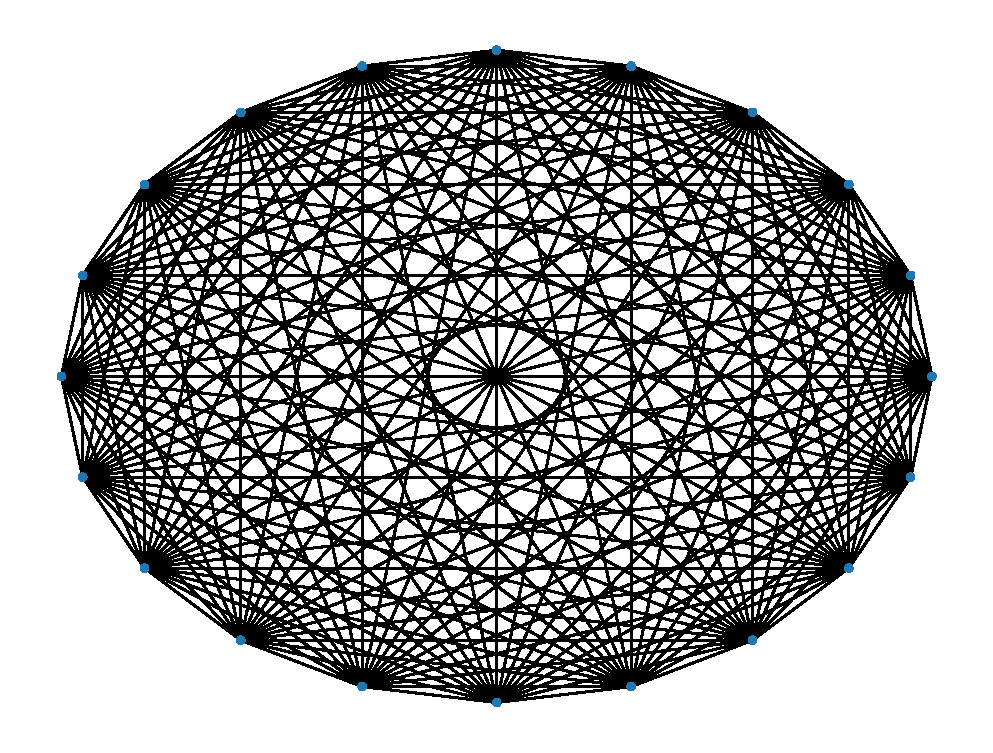
\includegraphics[width=0.6\textwidth]{completeGraph.eps}
    \caption{Plot of a complete circular graph with 20 nodes.}
    \label{circularGraph}
    
\end{figure}

\section{Topologies}

In this section we are going to discuss the classes that are implemented in the wrapper \textit{Topologies.py} and for the non-implemented codes the corresponding pseudocodes or reference will be presented. 

\subsection{Small World Network}

The implemented code is based on the Wattz-Strogatz Algorithm to create a small world network \cite{Watts1998}. First, we create an ordered network. Given \textit{N} nodes for each node we assign $K$ neigbors, half to the "left" and half to the "right". This could be understood in the following Figure. \ref{ordered}.

\begin{figure}[H]
    \centering
    \begin{tabular}{l l}
        a) & b) \\
        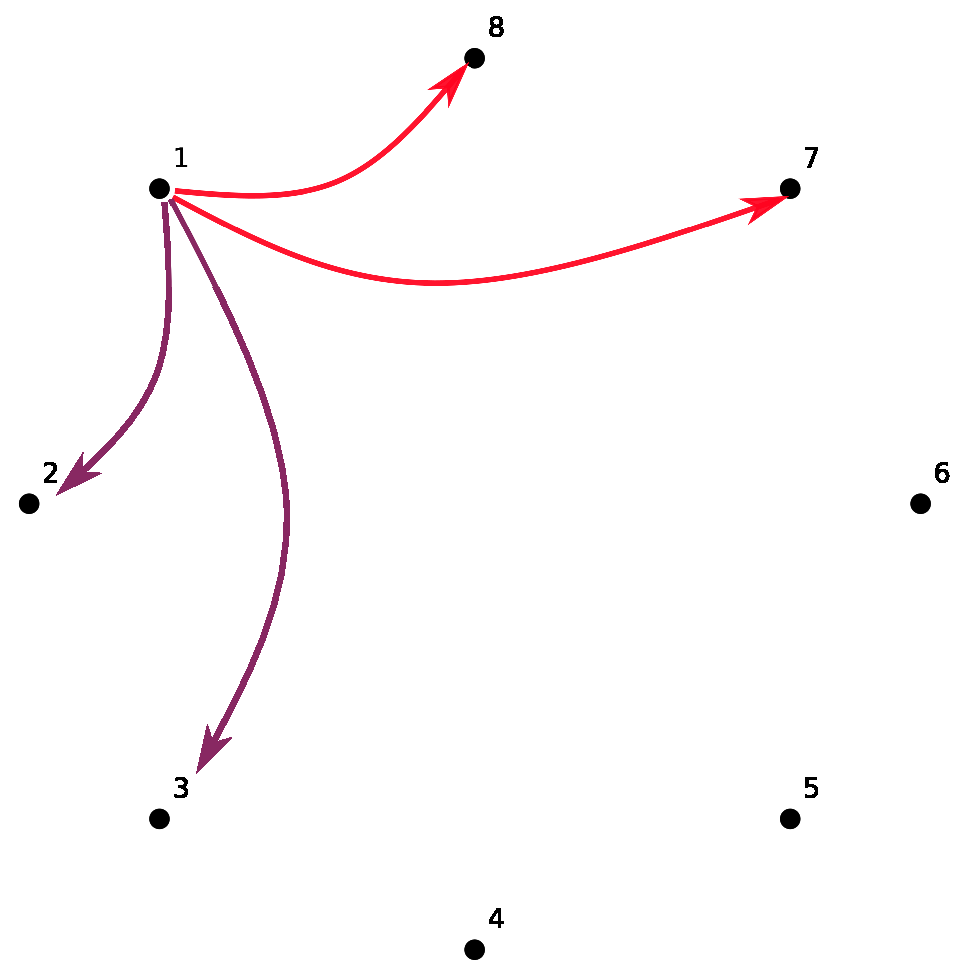
\includegraphics[width=0.5\textwidth]{empty.eps} &
        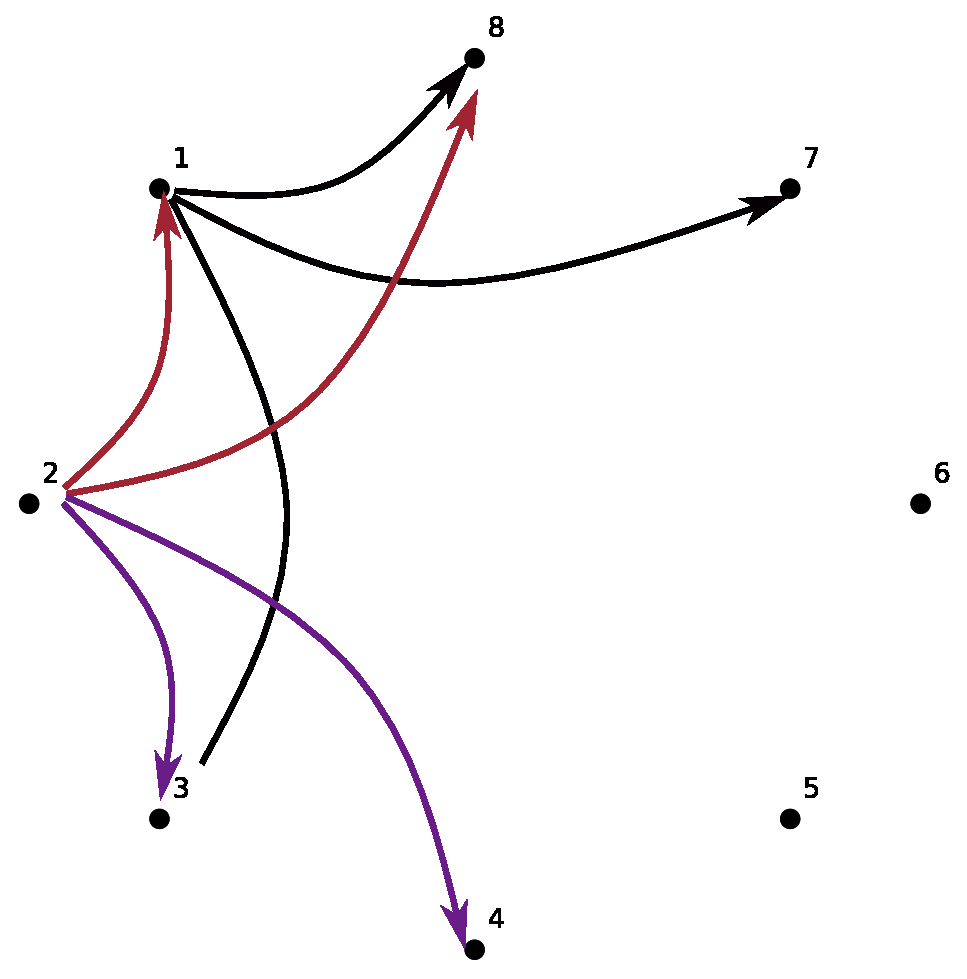
\includegraphics[width=0.5\textwidth]{empty2.eps}
    \end{tabular}
    \caption{Representation of the algorithm that create an ordered network with $K=4$ and $N=8$. a) Correspond to the first step of the algorithm. b) Second step of the algorithm. Red arrows correspond ot the left connections, purple arrows to right connections and black edges correspond to the connections of the previous step.}
    \label{ordered}
\end{figure}

Next, we proceed to scramble the network with probability $p$. Let consider the previous ordered network with $N=8$ and $K=4$ (Figure. \ref{ord}). 

\begin{figure}[H]
    \centering
    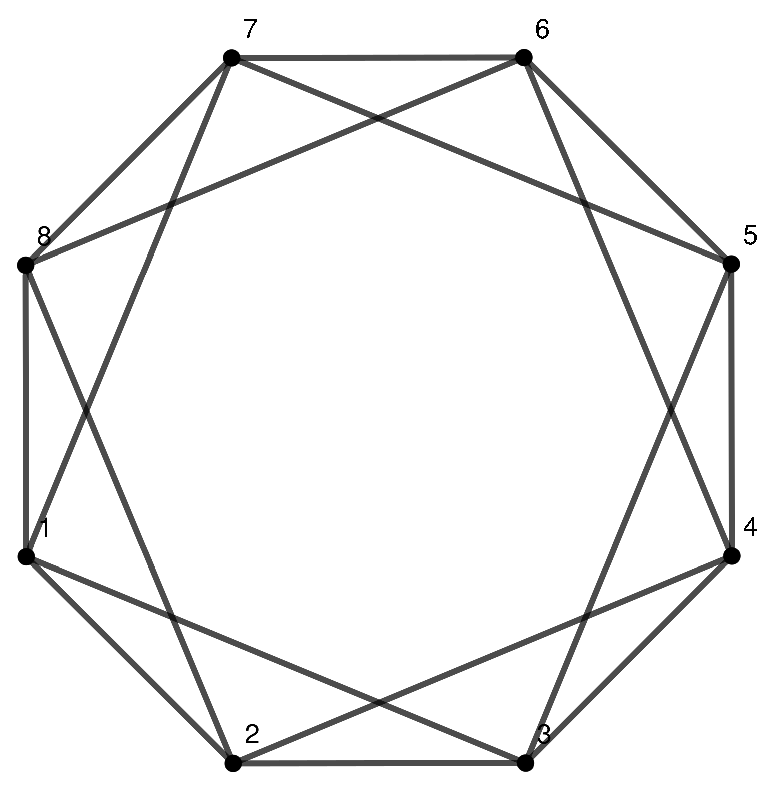
\includegraphics[width=0.8\textwidth]{ordered.eps}
    \caption{Ordered Graph with $K=4$ and $N=8$.}
    \label{ord}
\end{figure}

The algorithm "walks" through all the network and per each node $n_i$ it get a random number $r_i$ between $[0,1]$ and compare with $p$. If $r_i < p$, then it choose an aleatory neighbors from the right connections of $n_i.cnxL$ and reconnect with another node that is no in it connections of $n_i$. We repete the procedure with the next nodes. Notice that the scrambling or rewiring is performed in counterclockwise way (Figure. \ref{scram}).

\begin{figure}[H]
    \centering
    \begin{tabular}{l l}
        a) & b) \\
        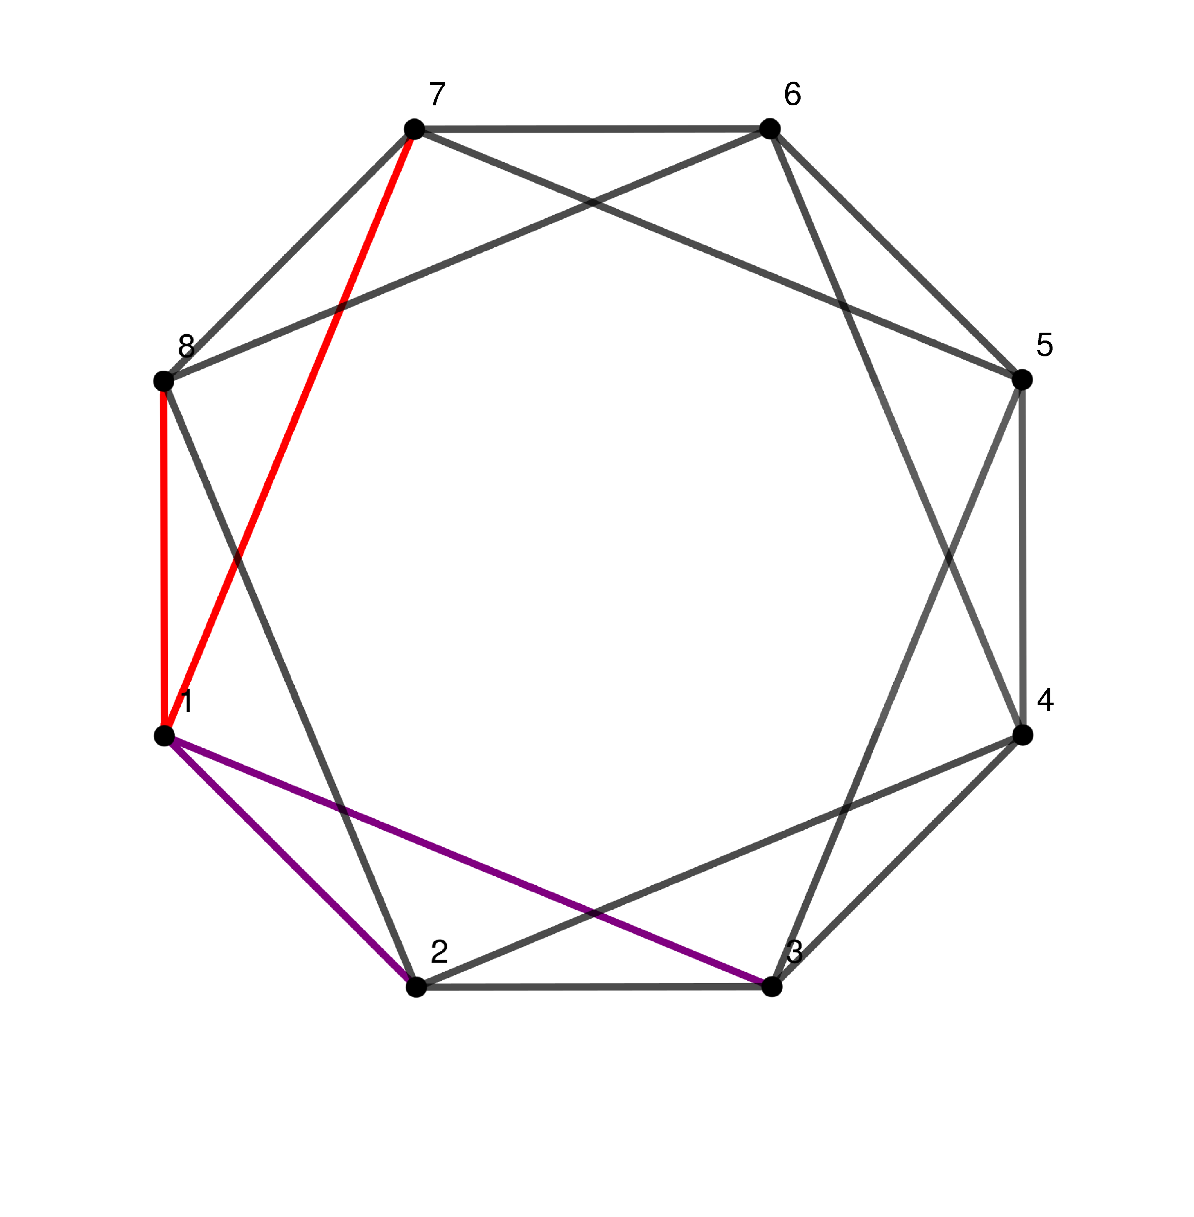
\includegraphics[width=0.55\textwidth]{scram.eps} &
        \includegraphics[width=0.45\textwidth]{scram2.eps}
    \end{tabular}
    \caption{Representation of the scrambling algorithm for a  network with $K=4$, $N=8$ and  probability $p$. a) Correspond to the ordered network. b) Correspond to the reconnection of the edge $1-3$ to $5$. Red edges correspond ot the left connections, purple edges to right connections and black edges correspond to the connections of the previous step.}
    \label{scram}
\end{figure}

\begin{lstlisting}[language=Python, caption= Small World Network Class]
from Node import node
from Network import network
import numpy as np
import matplotlib.pyplot as plt
import networkx as nx
import random


class nodeSW(node):
    
    def __init__(self, *argv):
        #Constructor of the node used in the Small world network algorithm. The right connections correspond to those that we are going to reconnect. The left connections correspond to those that are going to be eliminated.

        self.cnxL = argv[0]
        # Left connections 
        self.cnxR = argv[1]
        # Right connections 
        self.cnx = self.cnxL + self.cnxR
        # Total connections 

                        
class swNet(network):


    def __init__(self, NumeroNodos, K, p):
        """Constructor""" 
        self.N = NumeroNodos
        # Total Number of nodes
        self.nodetype = nodeSW
        # Type of node of the network
        self.nodes = self.orderedNetwork(K)
        # Create a ordered network
        self.wsNet(p)
        # Scramble the network 
        # #with a probability p
        

    def orderedNetwork(self, K):
        # Method to create an ordered network with
        # K number of neighbors per node
        # Input: K, number of neighbors
        # Outputs: List of objects self.nodetype

        totalN = self.N
        # total number of nodes
        nodesList = []
        # Initialice an empty list
        for i in range(totalN):
            nodo = self.nodetype([],[])
            nodesList.append(self.vecinos(nodo, i, K))
        # Append a class node with k neighbors; k/2 to left, k/2 to the right
        return nodesList

    def vecinos(self, nodo, i, K):
        # Method to assing the neigbors to a node
        # Input: nodo, class node
        #        i, the position of the node
        #        K, the total number of neighbors
        # Outputs: object self.typenode
                            
        totalN = self.N
        for j in range(K//2):
            nodo.cnxL.append((i-j-1)%totalN)
            # Assign the left connections
            nodo.cnxR.append((j+i+1)%totalN)
            # Assign the right connections
        self.actualizarcnx(nodo)
        # Update the state of the node 
        return nodo

    def actualizarcnx(self, nodo):
        # Method to update the total connections 
        # of a node
        # Input: object node
        nodo.cnx = nodo.cnxL + nodo.cnxR
        
        

    def printNodes(self):
        # Method to print the connections of all the nodes in the network
        for i in range(self.N):
            print("Nodo {}, {} ".format(i,self.nodes[i]))



    def wsNet(self, p):
        # Method to scramble an orderned network
        # with probability p
        # Input: p, float 
        # Output: updated network
        
        N=self.N
        # Total number of nodes
        for i in range(N):
        # We go through the network in counterclockwise direction, namely the from 0 to N. We assume that we had a circular network representation.
            rdm=random.random()
            # Get a random number between [0-1]
            if(rdm<p):
            # Verify if the random number is less than p
                n1=i 
                # Actual node
                n2=random.choice(self.nodes[n1].cnxR) 
                # Randomly we choose a connection to 
                # elminate
                n3=select_node(self.nodes[n1].cnx,n1,N) 
                # Randomly we choose a new connection

                self.nodes[n1].cnxR.remove(n2)
                self.nodes[n1].cnx.remove(n2)
                # Remove the connection n2 from n1
                self.nodes[n1].cnxL.append(n3)
                self.nodes[n1].cnx.append(n3)
                # Add the new connection n3 to n1
            
                self.nodes[n2].cnxL.remove(n1)
                self.nodes[n2].cnx.remove(n1)
                # Remove the node n1 from 
                # the connections of  n2
                
                self.nodes[n3].cnxL.append(n1)
                self.nodes[n3].cnx.append(n1)
                # Add the node n1 to n3

def select_node(cnxs,n1,N):
    # Function to choose a random node
    candidates=[]    
    for i in range(N):
        if (i not in cnxs) and (i != n1) :
            candidates.append(i)
    n2=random.choice(candidates)
    return n2
\end{lstlisting}

\subsection{Squared Network}

I could not find an pseudocode for this algorithm yet. Sorry. 

\subsubsection{Scale free Network}

I could not find an pseudocode for this algorithm yet. Sorry. Here you can find some of the models used \url{https://en.wikipedia.org/wiki/Scale-free_network}

\section{Dynamics}

In this section we are going to discuss the classes that are implemented in the wrapper \textit{Dynamics.py} and for the non-implemented codes the corresponding pseudocodes or reference will be presented. 

\subsection{Homophily}

In this subsection we are going to describe the first implemented dynamics. The Homophily dynamics consist on the tendency to relate with individuals that share the same attributes. In the implementation to complex networks, it means that our nodes should have attributes and the dynamics will consist on compare this attributes. The most simple model is consider a vector with $F$ attributes and $Q$ options to each attributes. For example for $F=3$  and $Q=2$ we could have the following vectors of attributes,

\begin{align*}
    vec1 &= \{1, 1,1 \}, \\
    vec2 &= \{0, 0,1 \}, \\
    vec3 &= \{0, 0,0 \},\\
    vec4 &= \{1, 0,1 \}, \\
    \vdots \quad &= \qquad.  \vdots
\end{align*}

Now, let us denote the set of neigbors of a node $n_i$ as $cnx_i$ and let us denote the vector of attributes associated to the node $n_i$ as $C_i = \left(\sigma_{i1},\sigma_{i2}, \dots , \sigma_{iF}  \right)$. In this way, the dynamics is described in the following way. First, for a node $n_i$ it is choose randomly a neighbor $n_j \in cnx_i$. Next, with a probability $$ p_{ij} = \frac{\sum_{k = 1}^{F}  \delta_{\sigma_{ik}, \sigma_{jk}}}{F}, $$
a random attribute of the node $n_i$ will adopt the attribute of the node $n_j$, namely $\sigma_{i \alpha} = \sigma_{j \alpha}$, where $\alpha$ is a random number between the attributes that are not the same (Figure. \ref{hom}).


\begin{figure}
    \centering
    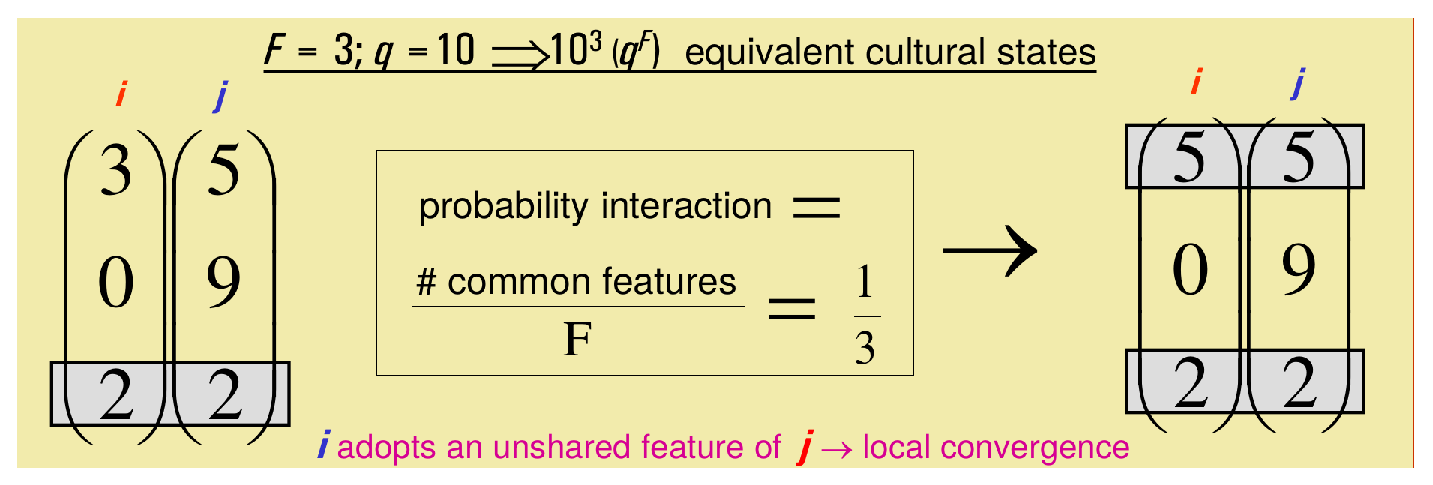
\includegraphics[width=0.8\textwidth]{hom.eps}
    \caption{Scheme of the homophily dynamics.}
    \label{hom}
\end{figure}

This procedure is repeated with all the nodes of the network independent of the topology.

Now, let us discuss the implementation of the code in python. This part could be a little bit confusing if you have any question or if you find a better implementation please let me know asap. We are taking advantages of OOP and the inherit characteristic of the classes. As it was presented in the general scheme of the software, we want that all the dynamics could be implemented independently of the topology of the network. In this sense, we define a new type of node $node_h$ that has a vector of parameter $vec_Param$ and the connections $cnx$. Then, in the dynamics, and for all the dynamics that we should implement, we create a method $initializer$ that given a network with an arbitrary topology it modify the type of node used in the network. Next, we define the constructor of the dynamics $homophily$, it have the type of node that we are going to use $node_type$; the total number of attributes $F$; the number of options per attribute $Q$; the number of attributes to adopt from the neighbor $n_ach$; the state of the network $net_state$ and the total time of simulation $T$. I have notice that this implementation could be improved in several ways, probably I will change somethings but this is illustrate the general idea of how to implement the dynamics. 


\begin{lstlisting}[language=Python, caption= Homophily Class]
# Module Homphile dynamics
from Topologies import *
from Node import node
import numpy as np
import matplotlib.pyplot as plt
import networkx as nx
import random


class node_H(node):

    def __init__(self, vect, cnxs):
        # Constructor of the node used in the
        # homophily dynamics
        # Inputs: vec_Param, a list of integers
        #         cnx, the list of neighbors
        self.vec_Param = vect
        self.cnx = cnxs 
        # List of neighbors of type node_H

class homophily:

    def __init__(self, net, parameters, options, nach, T):
        #Constructor of the homophily class
        # Inputs: 
        #   nodetype, specifies the type of node that 
        #             it is used
        #   F, the total number of parameters that each
        #       node have
        #   Q, the total number of options that each
        #      parameter have
        #   n_ach, the number of attributes to change
        #   net_state, is the state of the network at a #              given time
        #   T, the total time that the dynamics will run

        self.nodetype = node_H
        self.F = parameters
        self.Q = options
        self.n_ach = nach
        self.net_state = self.initializer(net)
        self.T = T

    def initializer(self, net):
        # Method that given a network with an arbitrary
        # topology it change the type of node. 
        # Input: net, a network with arbitrary topology
        # Output: the same network with different types 
        # or class of node. 

        N = net.N 
        #Total number of nodes
        for i in range(N):
            new_cnx = net.nodes[i].cnx
            parameters = self.parameters()
            # Generate the vector of parameter for each
            # node
            net.nodes[i] = self.nodetype(parameters, new_cnx)
            # modify the type of node in the network
        return net

    def parameters(self):
        # Method to randomly generate the vector of 
        # parameters of the nodes. 
        # Output: vect, a list of parameters of length
        # F with integers between [0,Q-1]
        opt = range(self.Q)
        total_elems = self.F
        vect = []
        for i in range(total_elems):
            vect.append(  random.choice(opt) )
        return vect


    def homophily_step(self):
        # Method tha apply the homophile dynamics for 
        # all the nodes of the network
        # Output: modifies the self.net_state
        N=self.net_state.N
        for i in range(N):
            self.node_hom(i)
            
            
            

    def node_hom(self, i):
        # Method tha implement the homophily dynamic 
        # per node
        # Input: i, index of the node
        # Output: modified node i
        
        n1=i 
        # node i
        n2=random.choice(self.net_state.nodes[n1].cnx)
        # Random neighbor of n1
    
        vec_sim= self.similarities(n1,n2)      
        # Obtain a bool vector. 1 equal. 0 diff.
        P=np.sum(vec_sim)/self.F   
        # Interaction probability
        
        if(random.random()<P):
            
            atrs_ch=select_atr(vec_sim, self.n_ach, self.F)  
            # Obtain the list of indeces of attributes to change
            
            for atr in atrs_ch:
            # Change the attributes of the node n1 as many times n_ach said    
                self.net_state.nodes[n1].vec_Param[atr]=self.net_state.nodes[n2].vec_Param[atr]
            

    def similarities(self, n1, n2):
        # Method that create a boolean vector of 
        # similarities between attributes of n1 and n2
        # Input: n1, n2 indexes of the nodes
        # Output: bec_s, boolean vector
        F= self.F
        vec_s=[]
        
        for i in range(F):
            if self.net_state.nodes[n1].vec_Param[i]==self.net_state.nodes[n2].vec_Param[i]:
                vec_s.append(1)
            else:
                vec_s.append(0)
        return vec_s

    def simulation(self):
        # Method that run a complet simulation of 
        # homophily dynamics with time T

        T_total = self.T

        for t in range(T_total):
            self.homophily_step()
            #print("time: {} Param  : {} \n".format(t, self.net_state.nodes[1].vec_Param))


def select_atr(vec_sim, n_ach, F):
    atrs_ch = []
    # Function to obtain the indixes of the attributes
    # to change
    not_eq= F-np.sum(vec_sim)
    if n_ach > not_eq:
        n_ach=not_eq
    
    candidates=[]
    
    for i in range(len(vec_sim)):
        if vec_sim[i]==0:
            candidates.append(i)
    
    for i in range(n_ach):
        selec=random.choice(candidates)
        atrs_ch.append(selec)
        candidates.remove(selec)
        
    return atrs_ch
\end{lstlisting}




\bibliographystyle{plain}
\bibliography{bibliography}

\end{document}
